\documentclass[12pt]{article}  % default square logo

\usepackage[margin=2.8cm]{geometry}
\usepackage{setspace}
\usepackage{mathptmx} % Times font
\usepackage{mathrsfs} % mathrsfs font
\usepackage{amsthm}   % theorems, definitions, lemmas

\usepackage{amsmath}  % \text{}
\usepackage[utf8]{inputenc}
\usepackage{graphicx}
\usepackage{framed} % frames
\usepackage{hyperref}
\usepackage{amssymb}  % empty set
\usepackage{multicol} % multi-column
\usepackage{tabu} % advanced table layout
\usepackage{chngcntr} % figure numbering per chapter
\usepackage{lib/bcprules} % typeset inference rule

% figure numbering
\counterwithin{figure}{section}

% code listing
\usepackage{listings}
\usepackage[table]{xcolor}

% packages for drawing
\usepackage{tikz}
\usetikzlibrary{graphs}     % create graphs
\usetikzlibrary{arrows}
\usetikzlibrary{trees}

%% set code styles

\definecolor{dkgreen}{rgb}{0,0.6,0}
\definecolor{gray}{rgb}{0.5,0.5,0.5}
\definecolor{shade}{rgb}{0.8,0.8,0.8}
\definecolor{mauve}{rgb}{0.58,0,0.82}

\lstset{
  % frame=tb,
  language=scala,
  aboveskip=3mm,
  belowskip=3mm,
  showstringspaces=false,
  columns=flexible,
  basicstyle={\small\ttfamily},
  numbers=none,
  numberstyle=\tiny\color{gray},
  keywordstyle=\color{blue},
  commentstyle=\color{dkgreen},
  stringstyle=\color{mauve},
  breaklines=true,
  breakatwhitespace=true,
  tabsize=3,
  xleftmargin=\parindent
}

% definitions, theorems

\theoremstyle{remark}
\newtheorem*{definition}{\textsc{Definition}}
\newtheorem*{theorem}{\textsc{Theorem}}
\newtheorem*{lemma}{\textsc{Lemma}}

\onehalfspacing

%end the preamble and start the document
\begin{document}

\begin{titlepage}

  \begin{center}

    %% \vspace{20cm}
    \vspace*{3\baselineskip}
    % Title
    {\Large A Study of Capability-based Effect Systems\\[2cm] }

    % Author and supervisor
    \noindent
    Fengyun Liu \\[2cm]

    \noindent
    A thesis submitted for the degree of \emph{Master of Computer
      Science} \\
    at École Polytechnique Fédérale de Lausanne \\[1.8cm]

    \noindent
    \begin{multicols}{3}
    Supervisor \\
    Martin Odersky \\
    Professor \\
    \vfill
    \columnbreak
    Mentor \\
    Nada Amin \\
    PhD \\
    \vfill
    \columnbreak
    Mentor \\
    Sandro Stucki\\
    PhD \\
    \end{multicols}

    \vspace*{3\baselineskip}

    \noindent
    {School of Computer and Communication Sciences \\[1cm]}
    % Upper part of the page. The '~' is needed because \\
    % only works if a paragraph has started.
    
\includegraphics[width=0.6\textwidth]{img/epfl}~\\[1cm]
    \noindent
    Lausanne, 2016 \\[1cm]

    %\vfill

    % Bottom of the page
    %% {\large \today}

  \end{center}

\end{titlepage}

%% \include{content/dedication}        % include a dedication.tex file
%% \include{content/acknowlegements}   % include an acknowledgements.tex file
\begin{abstract}
  Type-and-effect systems have been around for about thirty years. But
  they have never gained popularity in the programmer community,
  mainly due to the verbosity of its syntax. \emph{Monad-based} effect
  systems have a successful story in Haskell, but these systems can't
  handle \emph{effect polymorphism} well.

  % Haskell programmers often need to maintain two versions of the same
  % code, one is pure, the other is impure.

  In this study we took another approach and investigated
  \emph{capability-based} effect systems. In such systems, an instance
  of capability type is required to make side effects. For the system
  to work, we introduced \emph{stoic functions} which observe a
  \emph{variable-capturing} discipline, in contrast to \emph{free
    functions}, which has no contraints in capturing variables.

  Generally, capability-based effect systems are easier to understand
  and use than monads. Most importantly, powered by the combination of
  \emph{stoic functions} and \emph{free functions}, capability-based
  systems can quite well handle effect polymorphism. These merits make
  capability-based effect systems stand a better chance to be adopted
  by the programmer community.

  In this report we present four capability-based type-and-effect
  systems of increasing complexity, namely STLC-Pure, F-Pure,
  STLC-Impure and F-Impure. We proved soundness and effect safety for
  all the systems based on locally-nameless representation in Coq.

  % The system SLTC-Pure and F-Pure demonstrated that capability-based
  % effect systems can be used in pure functional languages to track
  % effects. The system STLC-Impure and F-Impure demonstrated that
  % capability-based effect systems can be used in a hybrid language
  % where only part of the program is effect-disciplined -- this
  % provides a flexibility to programmers when they don't care about
  % effects.

\end{abstract}
          % include the abstract

\tableofcontents            % generate and include a table of contents
% \listoffigures              % generate and include a list of figures

%now include the files of latex for each of the chapters etc
\section{Introduction}

The objective of this study is to explore the theoretical foundations
as well as conceptual possibilities of capability-based effect
systems. In this chapter, we'll discuss the motivation, the core ideas
and contributions of this study.

\subsection{Motivation}

The main motivation is to turn Scala into an effect-disciplined
programming language. Currently, Scala doesn't have the ability to
track effects in the type system. This poses a problem in distributed
and parallel programming. For example, in parallel computing, there's
often the need to stipulate that the functions passed to \emph{pmap}
have no side effects.

\begin{lstlisting}[language=Scala]
def pmap(xs: List[Int], f: Int => Int): List[Int]
\end{lstlisting}

However, currently it's impossible for the library author to impose
the constraint in the type system. A type-and-effect system has been
proposed for Scala\cite{lukas2014effect}, but is not well received in
the Scala community, mainly due to its notational verbosity in
handling \emph{effect polymorphism}. The problem of \emph{effect
  polymorphism} can be illustrated by the \emph{map} function:

\begin{lstlisting}[language=Scala]
  def map[A,B](f: A => B)(l: List[A]) = l match {
    case Nil => Nil
    case x::xs => f(x)::map(f)(l)
  }
\end{lstlisting}

In an effect system, the effect of \emph{map} depends on the passed in
function \emph{f}. If \emph{f} has IO effects, then \emph{map} also
has IO effects. If \emph{f} is pure, then \emph{map} is pure as
well. In order to make effect polymorphism work, proposed
type-and-effect systems usually require programmers to annotate the
function \emph{map} to say that its effect depends on the function
\emph{f}, which incurs some notational burden on programmers.

Monad-based effect systems have a success in Haskell. However, as we
will see, monad-based effect systems only work in lazy evaluation
languages, which is not a good fit for Scala because Scala is
strict. On the other hand, monad-based effect systems also face the
problem of \emph{effect polymorphism}. As reported in Chapter 1
section 6 of the thesis\cite{lippmeier2009type}, almost every general
purpose higher-order function in Haskell needs both a monadic version
and non-monadic version. For example, following code snippet shows the
signature for two versions of the \emph{map} function. The duplication
of code is a pity for programmers.

\begin{lstlisting}[language=Haskell]
  map :: (a -> b) -> List a -> List b
  mapIO :: (a -> IO b) -> List a -> IO (List b)
\end{lstlisting}

Given this situation, we are compelled to find a new approach to the
effect polymorphism problem, and \emph{capability-based} effect
systems seem to be a promising direction.

\subsection{Capability-based Effect Systems}

The central idea of \emph{capability-based} effect system is that an
instance of capability is required in order to make side effects. If
capabilities are passed as function parameters, by tracking
capabilities in the type system we can track effects in the program.

To ensure that capabilities are passed through function parameters,
instead of being captured from the environment, we need to impose a
\emph{variable-capturing discipline}, stipulating that capability
variables cannot be captured. Functions observe the discipline are
called \emph{stoic functions}, while functions don't oberve the
discipline are called \emph{free functions}.

With the combination of free functions and stoic functions,
\emph{capability-based} effect systems can solve the problem of
\emph{effect polymorphism} easily, while incurring no syntactical
burden. For example, instead of having two versions of \emph{map},
following \emph{map} is effect polymorphic.

\begin{lstlisting}[language=Scala]
  def map[A,B](f: A => B)(l: List[A]) = l match {
    case Nil => Nil
    case x::xs => f(x)::map(f)(l)
  }
\end{lstlisting}

When the passed function \emph{f} is pure, \emph{map} is pure as
well. In contrast, if \emph{f} is impure, then \emph{map} is also
impure. No additional annotation is required for effect polymorphism
to work. We'll see details of effect polymorphism in system
STLC-Impure.

\subsection{Contributions}

The main contributions of this study are as follows:

\begin{itemize}
\item Formulated and proved soundness and effect safety of four
  capability-based effect systems, which can serve as the fundation
  for implementing capability-based effect system in functional
  programming languages. The formalization is done in Coq based on the
  locally-nameless representation\cite{chargueraud-11-ln} and hosted
  on github\footnote{\url{https://github.com/liufengyun/stoic}}.
\item Proposed an approach to solve the problem of \emph{effect
    polymorphism} in capability-based effect systems with both free
  functions and stoic functions. The solution is much simpler and more
  elegant than in type-and-effect systems and monad-based effect
  systems.
\end{itemize}

\subsection{Structure of Report}

In following chapters, we'll introduce four systems of increasing
complexity, namely STLC-Pure, F-Pure, STLC-Impure and F-Impure.

\begin{itemize}
\item STLC-Pure is an variant of STLC with only stoic functions.
\item STLC-Impure is an extension of STLC-Pure with free functions and subtyping.
\item F-Pure is an extension of STLC-Pure with universal types.
\item F-Impure is an extension of F-Pure with free functions.
\end{itemize}

\section{System STLC-Pure}

This chapter describes a variant of the \emph{simply typed
  lambda calculus} with the extension of capabilities. We call this
system \emph{STLC-Pure}, because in this system all functions must
observe a variable-capturing discipline.

% In later chapters, we'll see the development of impure systems where
% there are both effect-disciplined functions which observe the
% variable-capturing discipline, and ordinary functions which don't
% observe the variable-capturing discipline.

The system STLC-Pure, though conceptually simple, can quite well
demonstrate the main features of capability-based effect
systems. We'll first introduce the formalization, then discuss
soundness and effect safety. Concepts introduced here will be a
foundation for more complex systems in later chapters.

\subsection{Definitions}

Formally, STLC-Pure is obtained by introducing a capability type and
imposing a variable-capturing discipline on lambda abstractions.
Figure~\ref{fig:stlc-pure-definition} presents the full definition of
STLC-Pure.

The syntax is almost the same as standard STLC, except the addition of
the capability type \emph{E} and the taking of variables as
values. The evaluation rules are exactly the same, with standard
call-by-value small-step semantics. The typing rule \textsc{T-Abs} is
slightly changed by performing an operation $pure$ on the
environment. The peculiarities in the formalization are explained
below.

\begin{figure}[h]
\begin{framed}

% multi-column separator
\setlength{\columnseprule}{0.4pt}
\begin{multicols}{2}

% \MTicinmath

\textbf{Syntax}

\begin{tabu} to \linewidth {l l l X[r]}
  $t$ & ::= &                     & terms:               \\
      &     & $x$                 & variable             \\
      &     & $\uplambda x{:}T.\, t$ & abstraction          \\
      &     & $t t$               & application          \\
\\
  $v$ & ::= &                        & values:              \\
      &     & $\uplambda x{:}T.\, t$ & abstraction value    \\
      &     & \colorbox{shade}{x}    & variable value       \\
\\
  $T$ & ::= &                      & types:               \\
      &     & $B$                  & basic type           \\
      &     & \colorbox{shade}{$E$}& capability type      \\
      &     & $T \to T$            & type of functions    \\
\end{tabu}

\hfill\\

\textbf{Evaluation} \hfill \framebox[1.2\width][r]{$t \longrightarrow t'$}

\infrule[E-App1]
{ t_1 \longrightarrow t'_1 }
{ t_1 \; t_2 \longrightarrow t'_1 \; t_2 }

\infrule[E-App2]
{ t_2 \longrightarrow t'_2 }
{ v_1 \; t_2 \longrightarrow v_1 \; t'_2 }

\infax[E-AppAbs]
{ (\uplambda x{:}T.\, t_1) v_2 \longrightarrow [x \mapsto v_2]t_1 }

\columnbreak

\textbf{Typing}  \hfill \framebox[1.2\width][r]{$\Gamma \vdash x : T$}

\infrule[T-Var]
{ x: T \in \Gamma }
{ \Gamma \vdash x : T }

\infrule[T-Abs]
{ \colorbox{shade}{$pure(\Gamma),\; x: S \vdash t_2 : T$} }
{ \colorbox{shade}{$\Gamma \vdash \uplambda x{:}S.\, t_2 : S \to T$} }

\infrule[T-App]
{ \Gamma \vdash t_1 : S \to T \andalso \Gamma \vdash t_2 : S }
{ \Gamma \vdash t_1 \; t_2 : T }

\colorbox{shade}{\textbf{Pure Environment}}

\hfill

\begin{center}
\begin{tabular}{l c l}
$pure(\varnothing)$      & = &  $\varnothing$ \\
$pure(\Gamma, \; x: E)$  & = &  $pure(\Gamma)$ \\
$pure(\Gamma, \; x: T)$  & = &  $pure(\Gamma), \; x: T$     \\
\end{tabular}
\end{center}

\end{multicols}
\end{framed}

\caption{System STLC-Pure}
\label{fig:stlc-pure-definition}
\end{figure}

\subsubsection{Variable-Capturing Discipline}

The most important change to the standard STLC lies in the following
typing rule:

\infrule[T-Abs]
{ pure(\Gamma), \; x: S \vdash t_2 : T }
{ \Gamma \vdash \uplambda x{:}S.t_2 : S \to T }

This typing rule imposes a \emph{variable-capturing discipline} on
lambda abstractions. This discipline stipulates that only variables
whose type is not a capability type can be captured in a lambda
abstraction.

The discipline is implemented with the helper function $pure$, which
removes all variable bindings of the capability type $E$ from the
typing environment. It's easy to verify that the function $pure$
satisfies following properties:

\begin{lemma}[Pure-Distributivity]
  pure ($\Gamma$, $\Delta$) = pure $\Gamma$, pure $\Delta$
\end{lemma}

\begin{lemma}[Pure-Idempotency]
  pure (pure $\Gamma$) = pure $\Gamma$
\end{lemma}

Initially, we've tried a variable-capturing discipline where no free
variables can be captured, i.e. $pure(\Gamma) = \varnothing$. While
this definition is certainly effect safe, the system is not very
expressive, as we lose the ability to create closures in the system,
which is usually considered to be an essential feature of functional
programming.

In addition to the capability type $E$, we also tried to exclude
variables of the type $T \to E$ (for any T) from the pure
environment. As an over-approximation, this version is certainly
effect-safe. However, it rejects more types than necessary, thus
reduces expressiveness of the system.

We introduce two useful definitions with the help of the function
$pure$.

\begin{definition}[Pure-Environment]
  An environment $\Gamma$ is pure if $pure \; \Gamma = \Gamma$.
\end{definition}

\begin{definition}[Pure-Type]
  A type is pure if the type can exist in a pure environment.
\end{definition}

From the definition, it's obvious that the type $B$ is pure, while $E$
is impure. However, a pure function type doesn't imply the
corresponding function is pure. For example, $E \to B$ is a pure type,
but functions that inhabit the type may have side effects, thus is
impure. The meta-theory of the system ensures that if the capability
type $E$ doesn't appear in the type signature of a function, then the
function must be pure. For example, all functions that can be typed as
$B \to B$ are guaranteed to be pure.

\subsubsection{Stoic Functions and Free Functions}

The variable-capturing discipline makes the functions in STLC-Pure
different from functions in standard STLC. In STLC, functions can
capture any variables in scope, while in STLC-Pure functions can only
capture variables whose type is not the capability type E. To
differentiate them (which is important as in later systems both
exist), we call the more effect-disciplined functions \emph{stoic
  functions} (or stoics) and the other \emph{free functions}. We use
$\to$ to denote the type of stoic functions and $\Rightarrow$ to
denote the type of free functions.

Stoic functions are essential in capability-based effect systems. If
functions are allowed to capture capability variables in scope, it
will be impossible to tell whether a function has side effect or not
(and what kind of effect) by just checking its type. Stoic functions
are effect-disciplined in the sense that the only way for stoic
functions to have side effects is to pass a capability as parameter,
thus it can be captured by the type system.

Stoic functions are not necessarily pure functions. Stoic functions
can have side effects, and if they do have side effects they are
honest about that in their type signature. For example, the following
function $hello$ is a stoic function with IO effects\footnote{For the
  sake of readability, we'll use a syntax similar to Scala in this
  report. In particular, we'll use $\to$ for the type of stoic
  functions, and $\Rightarrow$ for free functions.}.

\begin{lstlisting}[language=Scala]
  def hello(c:IO) = println("hello, world!", c)
\end{lstlisting}

In the following code snippet, the function $f$ must be pure, as it
doesn't take any capability as parameter. The type system guarantees
that the function indeed cannot produce any side effects.

\begin{lstlisting}[language=Scala]
  def twice(f: Int -> Int)(x: Int) = f (f x)
\end{lstlisting}

% In the functions passed, it's impossible to call functions to
% create side effects, as in STLC-Pure all functions that can have side
% effects take some capability as parameter.

\subsubsection{Where do Effects Come From}

There is no formalization of effects in the current effect system. We
assume the existence of primitive functions like $println$ and
$readln$, which take capabilities to produce side effects.

\begin{lstlisting}[language=Scala]
  def println: String -> IO -> ()
  def readln: IO -> String
\end{lstlisting}


% As the primary concern of this study is IO effects,

\subsubsection{Where do Capabilities Come From}

It is impossible to create capabilities in the current system. Where
do capabilities come from?  There are two possible answers: (1) all
capabilities are from the run-time and passed to the program through
the $main$ method; (2) there are no capabilities; they can be erased
before evaluation, without changing the meaning of programs.

% However, in this study we only state this observation informally and
% leave the formal proof to future studies.

\subsubsection{Why Treat Variables as Values}

As discussed above, there is no way to create a value of capabilities
explicitly. Thus, a function taking a parameter of the capability type
$E$ can never be executed in the \emph{call-by-value} semantics,
unless variables are values. The same is true for the base type $B$.

Treating variables as values ensures that substitution of a term with
a value of the base type $B$ or the capability type $E$ can actually
happen in the system, thus makes the preservation proof more
convincing.

% Adding variables as values doesn't break soundness or effect safety of
% the system. In fact, in adding variables as values, we only added 5
% lines of code in our soundness proof, and effect safety proof remains
% the same.

\subsubsection{What If a Function Has More than One Side Effect}

There is no support for a function with more than one kind of effects
in the current system. For example, in the following code snippet,
$c1$ cannot be used in the function body, as it's removed by $pure$ in
the typing of the function body.

\begin{lstlisting}[language=Scala]
  def error(e:Error)(c1:IO)(c2:Throw) = {
    println("error happen!", c1)  // Error, can't capture c1
    throw c2 e
  }
\end{lstlisting}

It's straight-forward to extend the system with pairs or tuples to
overcome this limitation. However, this is not an issue for later
systems with \emph{free functions}, thus we don't pursue the extension
of pairs and tuples here.

\subsection{Soundness}

\label{sec:stlc-pure-soundness}

We follow the standard formulation of soundness in TAPL
\cite{bpierce2002types}, which consists of \emph{progress} and
\emph{preservation}, defined as follows:

\begin{theorem}[Progress]
If $\varnothing \vdash t : T$, then either $t$ is a value or there is some
$t'$ with $t \longrightarrow t'$.
\end{theorem}

\begin{theorem}[Preservation]
If $\Gamma \vdash t : T$, and $t \longrightarrow t'$, then $\Gamma
\vdash t' : T$.
\end{theorem}

The proof of progress is the same as the proof in standard
STLC. However, there is a significant difference in the proof of
preservation. The classic proof of preservation for STLC (as shown in
TAPL) depends on a substitution lemma, which is formulated as follows:

\begin{lemma}[Subsitution-Classic]
If $\Gamma,\; x:S \vdash t : T$, and $\Gamma \vdash s : S$, then $\Gamma
\vdash [x \mapsto s]t : T$.
\end{lemma}

However, this substitution lemma doesn't hold in the current
system. For a counter-example, let's assume that
$\Gamma = \{f: E \to B,\; c:E\}$, then it's obviously that following
two typing relations hold:

$f: E \to B,\; c:E,\; x:B \vdash \uplambda z{:}B.\,x \; : \; B \to B$ \\
$f: E \to B,\; c:E \vdash f \; c \; : \; B$

However, the following typing relation doesn't hold if we replace $x$
with $f \; c$.

$f: E \to B,\; c:E \vdash \uplambda z{:}B.\,f \; c \; : \; B \to B$.

In fact, the substituted term $\uplambda z{:}B.\,f \; c$ cannot be
typed, as according to the typing rule \textsc{T-Abs}, it cannot
capture the capability variable $c$ in the environment. To overcome
this problem, we stipulate that the term $s$ must be a value. Remember
that in the current system, both lambda abstractions and variables are
values, thus substitution of variables of the capability type E and
the base type B can happen. The new formulation is as follows:

\begin{lemma}[Subsitution-New]
  If $\Gamma,\; x:S \vdash t : T$, s is a value and
  $\Gamma \vdash s : S$, then $\Gamma \vdash [x \mapsto s]t : T$.
\end{lemma}

The restriction that $s$ must be a value implies that in a function
call, arguments much first be evaluated to a value before the function
is applied. Therefore, capabilities can only work with strict
evaluation.

Interestingly, this strict evaluation requirement contrasts
capability-based effect systems with monad-based effect systems. In
Haskell, if strict evaluation is adopted, it will be impossible to
track effects in the type system, as demonstrated by the following
code snippet:

\begin{lstlisting}[language=Haskell]
  inc n = (\x -> n + 1) (putStrLn (show n))
\end{lstlisting}

The function $inc$ has the type
$(Num\;a, Show\;a) \Rightarrow a \to a$. By just checking its type, we
would think it has no side effects because no IO monads appear in the
type signature. However, if Haskell adopts strict evaluation, the
function call $putStrLn \; (show \; n)$ will be executed, thus
breaking the monad-based effect system.

\subsection{Effect Safety}

Does the system really work? This question prompts us to formulate and
prove effect safety of the system. We start by formulating effect
safety informally, then put forward a formal formulation, and finally
prove effect safety of the system.

\subsubsection{Informal Formulation}

A straight-forward violation of effect safety is for functions that
are taken as pure to have side effects inside the function body. Thus,
a tentative formulation would be as follows:

\begin{definition}[Effect-Safety-Informally-1]
A function typed in a pure environment cannot have side effects inside.
\end{definition}

However, this formulation is obviously problematic, as we know stoic
functions can have side effects if it takes a capability
parameter. Thus, we need to restrict the functions to those not taking
capability parameters:

\begin{definition}[Effect-Safety-Informally-2]
  A function, not taking any capability parameter and typed in a pure
  environment, cannot have side effects inside.
\end{definition}

This formulation looks more satisfactory, but it's a little
cumbersome. If we inspect the typing rule \textsc{T-Abs} closely, we
can find that if $S$ is not a capability type, $pure(\Gamma),\; x: S$
is equal to $pure(\Gamma,\; x: S)$.

\infrule[T-Abs]
{ pure(\Gamma),\; x: S \vdash t_2 : T }
{ \Gamma \vdash \uplambda x{:}S.\;t_2 : S \to T }

Thus, instead of saying the function $\uplambda x{:}S.\, t_2$ cannot
have side effects inside, we say the term $t_2$ cannot have side
effects in a pure environment. As we know, capabilities are required
to produce side effects. Thus, the term $t_2$ cannot have side effects
if we cannot construct a term of the capability type $E$ in a pure
environment. This observation leads us to the following statement of
effect safety:

\begin{definition}[Effect-Safety-Informally-3]
  It's impossible to construct a term of the capability type $E$ in a
  pure environment.
\end{definition}

However, this formulation cannot be proved.  For a counter-example,
let's assume $\Gamma = \{f: B \to E, \; x: B\}$. It's obvious that
$\Gamma$ is pure, but we can construct the term $f \; x$ of the
capability type $E$.

The cause of the problem is that in a pure environment, there might
exist non-inhabitable types like $B \to E$.  Existence of
non-inhabitable types in a pure environment doesn't pose a problem to
the system; a function taking a parameter of a non-inhabitable type
can never be actually called, thus is always effect-safe. So we only
need to consider environments with only variables of inhabitable
types.

To convince readers that the current system is effect-safe, we need to
exclude and only exclude non-inhabitable types from the pure
environment and then prove that it is impossible to construct a term
of the capability type $E$ in this restricted environment. We arrive
at the following formulation:

\begin{definition}[Effect-Safety-Informally-4]
  It's impossible to construct a term of the capability type $E$ in a
  pure environment with only variables of inhabitable types.
\end{definition}

\subsubsection{Inhabitability}

We need to define the concept \emph{inhabitability} precisely. What
types are inhabitable? Obviously, if $\varnothing \vdash t: T$, then
$T$ is inhabitable.  However, given a typing relation
$\Gamma \vdash t: T$, we cannot immediately conclude that $T$ is
inhabitable. We need to ensure that $\Gamma$ only contains inhabitable
types. Otherwise, any type is inhabitable if $\Gamma$ contains a
variable of the corresponding type.

An intuition is that, given $\Gamma \vdash t: T$, $x:S \in \Gamma$ and
$S$ is inhabitable, we can remove $x:S$ from $\Gamma$ and substitute
$x$ in the term $t$ with a witness of the type S to obtain a new term
$t'$. The substitution lemma tells us that the new term $t'$ still has
the type $T$. Continue this line of thought, we'll find out that all
inhabitable types can be inhabited in the empty environment. Thus, a
tentative definition is as follows:

\begin{definition}[Inhabitability-First-Try]
  A type $T$ is inhabitable if there exists a term $t$ with
  $\varnothing \vdash t : T$.
\end{definition}

However, this definition is not satisfactory in our case, as in
STLC-Pure there doesn't exist values for the base type $B$ and the
capability type $E$, except variables, and we do want both types to be
inhabitable. A natural approach is to extend the empty environment
with one variable of the base type and one of the capability type:

\begin{definition}[Inhabitability-Second-Try]
  A type $T$ is inhabitable if there exists a term $t$ with
  $x:B,\; y:E \vdash t : T$.
\end{definition}

This definition indeed gives us all inhabitable types in
STLC-Pure. Types like $E$, $B$, $E \to B$, $E \to E$,
$(B \to E) \to E$, etc., are all inhabitable, while types like
$B \to E$ and $E \to B \to E$ are non-inhabitable. The reader might
want to construct a witness of the type $B \to E$ as follows:

\begin{center}
  $x:B, \; y:E \vdash \uplambda x{:}B {.}\, y : B \to E$
\end{center}

The typing relation doesn't hold, because the typing rule
\textsc{T-Abs} would remove the binding $y:E$ from the environment in
the typing of the function body $y$.

The second formulation looks good, however, we can do better with the
following definition:

\begin{definition}[Inhabitability-Final]
  A type $T$ is inhabitable if there exists a value v with the typing
  $x:B, \; y:E \vdash v : T$.
\end{definition}

What if the term $t$ in the second definition is an application? In
that case, $t$ must be able to take a step until it becomes a value
due to \emph{progress} and \emph{normalization} of the
system\footnote{We didn't prove normalization of STLC-Pure, but the
  proof should be similar to the proof in standard STLC. We only
  proved progress in the empty environment, and the proof can be
  adapted to prove progress under $\{x:B, y:E\}$.}. And the
\emph{preservation} theorem tells us the type remains unchanged during
evaluation. This final definition makes proofs related to
inhabitability simpler. It's useful to give a definition of
inhabitable environments as well:

\begin{definition}[Inhabitable-Environment]
  An environment $\Gamma$ is inhabitable if it only contains variables
  of inhabitable types.
\end{definition}

\subsubsection{Formalization}

With the formal definition of inhabitability, we can formalize effect
safety as follows:

\begin{definition}[Effect-Safety-Inhabitability]
  If $\Gamma$ is a pure and inhabitable environment, then there
  doesn't exist $t$ with $\Gamma \vdash t : E$.
\end{definition}

However, this formulation doesn't give rise to a direct proof. In
fact, this statement is too strong. Some non-inhabitable types, such
as $E \to B \to E$, don't enable us to create a term of the type $E$,
thus it's safe to keep them in the environment. This implies it's
possible to impose a looser restriction on $\Gamma$, as long as all
types that can appear in a pure and inhabitable environment can also
appear in $\Gamma$.

When we examine the problem more closely, we found that through the
lens of the \emph{Curry-Howard isomorphism}, effect safety actually
says that it is impossible to prove the capability type $E$ from a
group of ``good'' premises. Thus, we can classify all types
(propositions) into two groups: in one group $E$ cannot be proved and
in the other group $E$ can be proved. This leads us to a formulation
of \emph{capsafe environment}\footnote{Sandro Stucki initially
  suggested the idea of using \emph{caprod} for the definition of
  \emph{pure} environments. I developed it to be a formulation of
  \emph{capsafe} environments and used it in the proof of effect
  safety.} given in Figure~\ref{fig:stlc-pure-capsafe-definition}. The
coined word \emph{capsafe} is an abbreviation of capability-safe, and
\emph{caprod} an abbreviation of capability-producing.

\begin{figure}[h]
\begin{framed}

% multi-column separator
\setlength{\columnseprule}{0.4pt}
\begin{multicols}{2}

\textbf{Capsafe Type}

\infax[CS-Base]
{ B \quad \text{capsafe} }

\infrule[CS-Fun1]
{ S \quad \text{caprod} }
{ S \to T \quad \text{capsafe} }

\infrule[CS-Fun2]
{ T \quad \text{capsafe} }
{ S \to T \quad \text{capsafe} }

\columnbreak

\textbf{Caprod Type}

\infax[CP-Eff]
{ E \quad \text{caprod} }

\infrule[CP-Fun]
{ S \; \text{capsafe} \andalso T \; \text{caprod} }
{ S \to T \quad \text{caprod} }

\textbf{Capsafe Environment}

\infax[CE-Empty]
{ \varnothing \quad \text{capsafe} }

\infrule[CE-Var]
{ \Gamma \; \text{capsafe} \andalso T \; \text{capsafe} }
{ \Gamma, \; x:T \quad \text{capsafe} }


\end{multicols}
\end{framed}

\caption{System STLC-Pure Capsafe Environment}
\label{fig:stlc-pure-capsafe-definition}
\end{figure}

In the definition, types like $B \to B$, $E \to E$, $E \to B$ and
$(B \to E) \to B$ are considered as \emph{capsafe}, while types like
$B \to E$, $(E \to B) \to E$ are considered as \emph{caprod}. Only
\emph{capsafe} types can appear in a \emph{capsafe} environment. To
inspect the formalization in detail, we can ask several questions.

\emph{Are capsafe types inhabitable?} The answer is not
necessarily. The type $E \to B \to E$ is capsafe but
non-inhabitable. Allowing this type in the capsafe environment doesn't
enable us to construct a term of the capability type $E$.

\emph{Are inhabitable types capsafe?} The answer is yes, except the
capability type $E$. As the capability type $E$ cannot appear in the
pure environment, this is not a problem.

\emph{Are caprod types non-inhabitable?} Yes, except the capability
type $E$. As $E$ is also excluded in the pure environment, it's
justified to remove it from the capsafe environment.

% Intuitively, the rule \textsc{CP-Fun} can be justified by the fact
% that in a capsafe environment it is impossible to construct a function
% which takes a \emph{capsafe} parameter and returns a value of
% \emph{caprod} type. Or from a logical point of view, given a proof
% from which E cannot be proved, we cannot transform it to be a proof
% capable of proving E, together with a group of premises incapable of
% proving E.

Why this formulation of capsafe environment is acceptable? In short,
it is because the statement \emph{Effect-Safety-Inhabitability} is
logically implied by the more general statement \emph{Effect-Safety}:

\begin{definition}[Effect-Safety]
  If $\Gamma$ is capsafe, then there doesn't exist $t$ with
  $\Gamma \vdash t : E$.
\end{definition}

The logical implication holds because a pure and inhabitable
environment is also a capsafe environment. This claim has been
formally proved:

\begin{lemma}[Inhabitable-Capsafe]
  If the type $T$ is inhabitable, then either $T$ is capsafe or $T = E$.
\end{lemma}

\begin{theorem}[Inhabitable-Pure-Capsafe-Env]
  If $\Gamma$ is pure and inhabitable, then $\Gamma$ is capsafe.
\end{theorem}

% From the theorem above, it's obvious that any property proved for a
% capsafe environment also holds for a pure and inhabitable
% environment. Therefore, it suffices to prove the statement
% \emph{Effect-Safety}.

\subsubsection{Proof}

The proof of effect safety depends on following lemmas, most of them
are straight-forward to prove. Effect safety follows immediately from
the lemma \emph{Capsafe-Env-Capsafe}.


\begin{lemma}[Capsafe-Not-Caprod]
 If type $T$ is capsafe, then $T$ is not caprod.
\end{lemma}

\begin{lemma}[Capsafe-Or-Caprod]
 For any $T$, $T$ is either capsafe or caprod.
\end{lemma}

\begin{lemma}[Capsafe-Env-Capsafe]
  If $\Gamma$ is capsafe and $\Gamma \vdash t : T$, then $T$ is capsafe.
\end{lemma}

\begin{theorem}[Effect-Safety]
  If $\Gamma$ is capsafe, then there doesn't exist $t$ with
  $\Gamma \vdash t : E$.
\end{theorem}

\subsubsection{An Intuitive Proof}

There exists an intuitive proof of effect safety without resorting to
capsafe environments. The main insight is that the statement
\emph{Effect-Safety-Inhabitability} is logically implied by the
statement \emph{Effect-Safety-Intuitive}:

\begin{definition}[Effect-Safety-Inhabitability]
  If $\Gamma$ is a pure and inhabitable environment, then there
  doesn't exist $t$ with $\Gamma \vdash t : E$.
\end{definition}

\begin{definition}[Effect-Safety-Intuitive]
  There doesn't exist value $v$ with $x:B \vdash v : E$.
\end{definition}

The statement \emph{Effect-Safety-Intuitive} trivially holds, because
the value $v$ can either be a variable or a function, in neither case
can it be typed as the capability type $E$.

Why does the logical implication hold? In short, if
\emph{Effect-Safety-Inhabitability} doesn't hold, then
\emph{Effect-Safety-Intuitive} doesn't hold either. Thus, the latter
logically implies the former.  In the following, we present an
informal proof, the core idea that if $\Gamma$ is pure and
inhabitable, and $\Gamma \vdash t : E$, then we can ``collapse''
$\Gamma$ to $\{b : B\}$ through substitution of the witnesses of the
pure and inhabitable types in $\Gamma$.

For a pure and inhabitable environment
$\Gamma = \{x:T, \; y:S, \; \dots, \; z:U\}$, if there exists $t$ with
$\Gamma \vdash t : E$, then the typing relation still holds by
extending the environment with $b:B$:

\begin{center}
$b:B, \; x:T, \; y:S, \; \dots, \; z:U \vdash t: E$
\end{center}

The type $U$ is pure and inhabitable, as $\Gamma$ is pure and
inhabitable. According to the definition of \emph{inhabitability},
there exists a value $u$ with $b:B, \; e:E \vdash u: U$. As $u$ is a
value, it can be either a variable or a function. If $u$ is a
variable, it can only be $b$, as $U$ is a pure type and the variable
$e$ binds to the impure capbility type $E$. If $u$ is a function, we
have $b:B \vdash u: U$, as in the typing of stoic functions the rule
\textsc{T-Abs} will remove the binding $e:E$ from the environment. In
both cases, we have $b:B \vdash u: U$. Now using the substitution
lemma, we have:

\begin{center}
$b:B, \; x:T, \; y:S, \; \dots \vdash [z \mapsto u]t: E$
\end{center}

Continue this process, we can reduce the typing environment to be
$\{b:B\}$ and the term to $t'$:

\begin{center}
$b:B \vdash t': E$
\end{center}

Now combining \emph{progress} and \emph{normalization} of
STLC-Pure\footnote{We only proved that progress holds in an empty
  environment, it's easy to prove it also holds under $\{b:B\}$. We
  didn't prove normalization of STLC-Pure, but the proof should be
  similar to the proof in standard STLC.}, $t'$ can take finite
evaluation steps to become a value $v$:

\begin{center}
$b:B \vdash v: E$
\end{center}

To summarize, we have given an intuitive proof of the following
statement:

\begin{center}
  $\neg \; \text{Effect-Safety-Inhabitability} \to \neg \;
  \text{Effect-Safety-Intuitive}$
\end{center}

By the logical law \emph{contraposition}, we have:

\begin{center}
  $ \text{Effect-Safety-Intuitive} \to
  \text{Effect-Safety-Inhabitability} $
\end{center}

As \emph{Effect-Safety-Intuitive} trivially holds,
\emph{Effect-Safety-Inhabitability} follows by \emph{modus ponens}.

Though conceptually simpler, the mechanized proof necessitates the
proof of the normalization theorem, which is more involved than the
proof based on capsafe environments. On the other hand, the approach
based on capsafe environments works even if normalization doesn't
hold. Therefore, we don't take the intuitive approach in the formal
development.

% extensions and practicality

\section{System F-Pure}

In this chapter, we present the system \emph{F-Pure}, which is an
extension of the system STLC-Pure with universal types. In this
system, not only functions need to observe a variable-capturing
discipline, type abstractions also need to observe the same
variable-capturing discipline.

We'll first introduce the formalization, then discuss soundness and
effect safety. In the discussion, we'll focus on its difference from
the system STLC-Pure.

\begin{figure}
\begin{framed}

% multi-column separator
\setlength{\columnseprule}{0.4pt}
\begin{multicols}{2}

\textbf{Syntax}

\begin{tabu} to \linewidth {l l l X[r]}
  t   & ::= &                                      & terms:               \\
      &     &  x                                   & variable             \\
      &     & $\lambda$ x:T.t                      & abstraction          \\
      &     & t t                                  & application          \\
      &     & \colorbox{shade}{$\lambda$ X.t}      & type abstraction     \\
      &     & \colorbox{shade}{t [T]}              & type application     \\
\\
  v   & ::= &                    & values:              \\
      &     & $\lambda$ x:T.t    & abstraction value    \\
      &     & x                  & variable value       \\
      &     & \colorbox{shade}{$\lambda X.t$}    & type abstraction value  \\
\\
  T   & ::= &                       & types:               \\
      &     & \colorbox{shade}{X}   & type variable        \\
      &     & B                     & basic type           \\
      &     & E                     & capability type      \\
      &     & T $\to$ T             & type of functions    \\
      &     & \colorbox{shade}{$\forall$ X.T} & universal type       \\
\end{tabu}

\hfill\\

\textbf{Evaluation} \hfill \framebox[1.2\width][r]{$t \longrightarrow t'$}

\infrule[E-App1]
{ t_1 \longrightarrow t'_1 }
{ t_1 \; t_2 \longrightarrow t'_1 \; t_2 }

\infrule[E-App2]
{ t_2 \longrightarrow t'_2 }
{ v_1 \; t_2 \longrightarrow v_1 \; t'_2 }

\infax[E-AppAbs]
{ (\lambda x:T.t_1) v_2 \longrightarrow [x \mapsto v_2]t_1 }

\infrule[E-TApp]
{ \colorbox{shade}{$t_1 \longrightarrow t'_1$} }
{ \colorbox{shade}{$t_1 \; [T_2] \longrightarrow t'_1 \; [T_2]$} }

\infax[E-TappTabs]
{ \colorbox{shade}{$(\lambda X.t_1) [T_2] \longrightarrow [X \mapsto T_2]t_1$} }

\columnbreak

\textbf{Typing}  \hfill \framebox[1.2\width][r]{$\Gamma \vdash x : T$}

\infrule[T-Var]
{ x: T \in \Gamma }
{ \Gamma \vdash x : T }

\infrule[T-Abs]
{ pure(\Gamma),\; x: S \vdash t_2 : T }
{ \Gamma \vdash \lambda x:S.t_2 : S \to T }

\infrule[T-App]
{ \Gamma \vdash t_1 : S \to T \andalso \Gamma \vdash t_2 : S }
{ \Gamma \vdash t_1 \; t_2 : T }

\infrule[T-TAbs]
{ \colorbox{shade}{$pure(\Gamma),\; X \vdash t_2 : T$} }
{ \colorbox{shade}{$\Gamma \vdash \lambda X.t_2 : \forall X. T$} }

\infrule[T-TApp]
{ \colorbox{shade}{$\Gamma \vdash t_1 : \forall X.T \andalso T_2 \neq E$} }
{ \colorbox{shade}{$\Gamma \vdash t_1 \; [T_2] : [X \mapsto T_2]T$} }

\hfill\\

\textbf{Pure Environment}

\hfill

\begin{center}
\begin{tabular}{l c l}
pure($\varnothing$)             & = &   $\varnothing$ \\
pure($\Gamma$, x: E)            & = &  pure($\Gamma$) \\
pure($\Gamma$, x: T)  & = &  pure($\Gamma$), x: T     \\
\rowcolor{gray!40}
pure($\Gamma$, X)  & = &  pure($\Gamma$), X  \\
\end{tabular}
\end{center}


\end{multicols}
\end{framed}

\caption{System F-Pure}
\label{fig:f-pure-definition}
\end{figure}

\subsection{Definitions}

The system F-Pure extends STLC-Pure with universal
types. Figure~\ref{fig:f-pure-definition} presents the full definition
of F-Pure, with the difference from the system STLC-Pure highlighted.

The extension of syntax and evaluation rules are exactly the same as
the extension of standard STLC with universal types.  The essential
difference lies in the two new typing rules \textsc{T-TAbs} and
\textsc{T-TApp}. The typing rule \textsc{T-TAbs} stipulates that type
abstraction must observe the variable-capturing discipline.

\infrule[T-TAbs]
{ pure(\Gamma),\; X \vdash t_2 : T }
{ \Gamma \vdash \lambda X.t_2 : \forall X. T }

We made this design choice in order to allow universal types to be
present in pure environments. Otherwise, if type abstractions can
capture capability variables, application of a type abstraction could
generate a term of the capability type or have side effects. This
makes it incorrect to have universal types in pure environments, thus
renders universal types useless in the system.

The typing rule \textsc{T-TApp} requires that the type parameter
cannot be the capability type E. However, it's allowed to supply
non-inhabitable types like $B \to E$ as parameter to type abstraction.

% This restriction implies in system F-Pure polymorphism doesn't cover
% capability types.

\infrule[T-TApp]
{ \Gamma \vdash t_1 : \forall X.T \andalso T_2 \neq E }
{ \Gamma \vdash t_1 \; [T_2] : [X \mapsto T_2]T }

Without the restriction, preservation of the system breaks, as can be
seen from following term $t$, which has the type
$\forall T. T \to B \to T$:

\begin{center}
  $t = \lambda T. \; \lambda x:T. \; \lambda y:B. \; x$
\end{center}

If we allow $E$ as parameter to type application, the term $t [E]$
would have the type $E \to B \to E$. However, after one evaluation
step, the term $\lambda x:E. \; \lambda y:B. \; x$ cannot be typed
anymore, as the capability variable $x$ cannot be captured in the
inner-most lambda; thus preservation breaks.

The definition of the function \emph{pure} is changed slightly by
allowing type variables to be in the pure environment. This is
natural, as we know in the typing rule \textsc{T-TApp} that a type
variable cannot be of the capability type.

\subsection{Soundness}

We proved both progress and preservation of the system.

\begin{theorem}[Progress]
If $\varnothing \vdash t : T$, then either $t$ is a value or there is some
$t'$ with $t \longrightarrow t'$.
\end{theorem}

\begin{theorem}[Preservation]
If $\Gamma \vdash t : T$, and $t \longrightarrow t'$, then $\Gamma
\vdash t' : T$.
\end{theorem}

The proof of progress is the same as in System F. In the proof of
preservation, we need to make small changes to the standard
substitution lemmas in System F.

\begin{lemma}[Subsitution-Term]
  If $\Gamma,\; x:S \vdash t : T$, s is a value and
  $\Gamma \vdash s : S$, then $\Gamma \vdash [x \mapsto s]t : T$.
\end{lemma}

\begin{lemma}[Subsitution-Type]
  If $\Gamma,\; X \vdash t : T$ and P $\neq$ E,
  then $\Gamma \vdash [X \mapsto P]t : [X \mapsto P]T$.
\end{lemma}

We restrict $s$ to be a value in the lemma \emph{Substitution-Term}
for the same reason as in the system STLC-Pure. In the lemma
\emph{Substitution-Type}, we restrict that $P$ is not the capability
type E. Otherwise, the lemma cannot be proved as explained in the
previous section.

\subsection{Effect Safety}

We follow the same approach as in the system STLC-Pure in the
formulation of effect safety.

\subsubsection{Inhabitability}

In the presence of universal types, we need to adapt the definition of
inhabitable types and inhabitable environments.

The definition of inhabitable environment in STLC-Pure would reject a
well-formed environment with type variables like
$\{T, S, f: T \to S, x:T\}$, which could be the environment for
the following well-defined function:

\begin{lstlisting}[language=Scala]
  def apply[T, S](f: T -> S)(x: T) = f x
\end{lstlisting}

To handle this problem, we propose the definition of \emph{inhabitable
  types} and \emph{inhabitable environment} as shown in
Figure~\ref{fig:f-pure-inhabitability}.

\begin{figure}[h]
\begin{framed}

% multi-column separator
\setlength{\columnseprule}{0.4pt}
\begin{multicols}{2}

\textbf{Primitive Environment}

\infax[P-Base]
{ x:B, \; y:E \quad primitive }

\infrule[P-TVar]
{ \Sigma \quad primitive }
{ \Sigma ,\; X \quad primitive }

\infrule[P-Type]
{ \Sigma \quad primitive }
{ \Sigma ,\; x:X \quad primitive }

\textbf{Inhabitable Type}

\infrule[IT]
{\Sigma \; primitive \andalso \Sigma \vdash v : T}
{ T \quad inhabitable }

\columnbreak

\textbf{Inhabitable Environment}

\infax[IE-Empty]
{ \varnothing \quad inhabitable }

\infrule[IE-TVar]
{ \Gamma \quad inhabitable }
{ \Gamma ,\; X \quad inhabitable }

\infrule[IE-Type]
{ \Gamma \; inhabitable \andalso T \; inhabitable   }
{ \Gamma ,\; x:T \quad inhabitable }

\end{multicols}
\end{framed}

\caption{System F-Pure Inhabitable Environments }
\label{fig:f-pure-inhabitability}
\end{figure}

The definition of inhabitable types depends on \emph{primitive
  environments}. A primitive environment is the extension of the
environment $\{x:B, y:E\}$ with any type variables and type variable
bindings. This definition would take types like $X$, $X \to Y$ as
inhabitable, as expected.

The definition of inhabitable environment not only allow bindings of
inhabitable types, but also allow any type variables to be present in
an inhabitable environment. This definition ensures that only
non-inhabitable types, such as $B \to E$, $\forall X.X$ and
$\forall X.\forall Y.X \to Y$ are rejected from pure environments.

\subsubsection{Formulation}

As in STLC, the standard formulation is given based on inhabitable
environments:

\begin{definition}[Effect-Safety-Inhabitability]
  If $\Gamma$ is a pure and inhabitable environment, then there
  doesn't exist $t$ with $\Gamma \vdash t : E$.
\end{definition}

The proof of the statement depends on a weaker and more general
statement about \emph{healthy environments}. If we can arrive at such
a definition of \emph{healthy environment} that a pure and inhabitable
environment is also healthy, then it suffices to prove the following
statement about healthy environments:

\begin{definition}[Effect-Safety]
  If $\Gamma$ is healthy, there doesn't exist $t$ with
  $\Gamma \vdash t : E$.
\end{definition}

What \emph{capsafe} and \emph{caprod} rules we need for universal
types? Obviously, we need to take the non-inhabitable type
$\forall X.X$ as \emph{caprod}, as with a variable of this type, it's
possible to create a term of the capability type E. For example, if
$x$ is of the type $\forall X.X$ and $b$ is of the type $B$, then
$x \; [B \to E] \; b$ has the type $E$.  We also need to take the
non-inhabitable type $\forall X. \forall Y. X \to Y$ as
\emph{caprod}. Otherwise, if $x$ is of the type
$\forall X. \forall Y. X \to Y$ and $b$ is of the type $B$, then
$x \; [B] \; [B \to E] \; b \; b$ has the type $E$. This observation
leads us to following rules for universal types.

\infrule[CS-All]
{ [X \mapsto B]T \; \text{capsafe} \andalso [X \mapsto E]T \; \text{capsafe} }
{ \forall X.T \quad \text{capsafe} }

\infrule[CP-All]
{ [X \mapsto B]T \; caprod \quad or \quad [X \mapsto E]T \; caprod }
{ \forall X.T \quad caprod }

% We need to ensure that thew new rule CP-All only mark non-inhabitable
% types as $caprod$. As before, we only provide informal argument
% here. The justification for the rule \text{CP-All} is that, if a
% universal type is inhabitable, then it must be inhabitable by
% replacing the type parameter with any type (except E). Thus if a
% specialized universal type is caprod (which we know is non-inhabitable
% as argued before), then the universal type is also
% non-inhabitable. Therefore, the \textsc{CP-All} rule only marks
% non-inhabitable types as caprod.

% Note that in the explanation above, we say that the capability type E
% is an exception. For example, the type $\forall T.T \to B \to T$ is
% inhabited by the term
% $\lambda T. \; \lambda x:T. \; \lambda y:B. \; x$. However, the type
% $E \to B \to E$ is non-inhabitable. This is not a problem since
% $E \to B \to E$ is \emph{capsafe}. In fact, in the initial
% formulation, we used $B \to E$ instead of $E$ in \textsc{CS-All} and
% \textsc{CP-All}. Later, we found out that we can simplify the
% formulation without changing the proof of effect safety.

The full definition of the \emph{healthy environment} is presented in
Figure~\ref{fig:f-pure-healthy-definition}, with difference from
STLC-Pure highlighted.

\begin{figure}[h]
\begin{framed}

% multi-column separator
\setlength{\columnseprule}{0.4pt}
\begin{multicols}{2}

\textbf{Capsafe}

\infax[CS-Base]
{ B \quad \text{capsafe} }

\infrule[CS-Fun1]
{ S \quad caprod }
{ S \to T \quad \text{capsafe} }

\infrule[CS-Fun2]
{ T \quad \text{capsafe} }
{ S \to T \quad \text{capsafe} }

\infrule[CS-All]
{ \colorbox{shade}{$[X \mapsto B]T \; \text{capsafe} \andalso [X \mapsto E]T \; \text{capsafe}$} }
{ \colorbox{shade}{$\forall X.T \quad \text{capsafe}$} }

\columnbreak

\textbf{Caprod}

\infax[CP-Eff]
{ E \quad caprod }

\infrule[CP-Fun]
{ S \; \text{capsafe} \andalso T \; caprod }
{ S \to T \quad caprod }

\infrule[CP-All]
{ \colorbox{shade}{$[X \mapsto B]T \; caprod \quad or \quad [X \mapsto E]T \; caprod$} }
{ \colorbox{shade}{$\forall X.T \quad caprod$} }

\textbf{Healthy}

\infax[H-Empty]
{ \varnothing \quad caprod }

\infrule[H-Var]
{ G \; healthy \andalso T \; \text{capsafe} }
{ G, \; x:T \quad healthy }

\infrule[H-TVar]
{ \colorbox{shade}{$G \quad healthy$} }
{ \colorbox{shade}{$G, \; X \quad healthy$} }

\hfill\\

\end{multicols}
\end{framed}

\caption{System F-Pure Healthy Environment}
\label{fig:f-pure-healthy-definition}
\end{figure}

Why this formulation of healthy environment is acceptable? In short,
it's because the statement \emph{Effect-Safety} logically implies the
statement \emph{Effect-Safety-Inhabitability}.

The logical implication holds because a pure and inhabitable
environment is also a healthy environment. This claim has been
formally proved:

\begin{theorem}[Inhabitable-Capsafe]
  If the type T is inhabitable, then either T is capsafe or $T = E$.
\end{theorem}

\begin{theorem}[Inhabitable-Pure-Healthy]
  If $\Gamma$ is pure and inhabitable, then $\Gamma$ is also healthy.
\end{theorem}

% From the theorem above, it's obvious that any property proved for a
% healthy environment also holds for a pure and inhabitable
% environment. Thus, it suffices to prove the statement
% \emph{Effect-Safety}

\subsubsection{Proof}

The proof of effect safety is more involved than in STLC-Pure. We need
to introduce the \emph{degree} of types in the proof of
relevant lemmas about types.

\begin{definition}[Degree of Type]
  The degree of a type $T$ is defined as follows:
  \begin{equation*}
    degree(T) =
    \begin{cases}
      max(degree(t_1), degree(t_2)) & \text{if } T = T_1 \to T_2,\\
      degree(T_1) + 1 & \text{if } T = \forall X.T_1,\\
      0 & others
    \end{cases}
  \end{equation*}
\end{definition}

With the help of the definition above, it's possible to prove
following lemmas based on double induction on the degree of types and
the type T.

\begin{lemma}[Capsafe-Not-Caprod]
 If type T is capsafe, then T is not caprod.
\end{lemma}

\begin{lemma}[Capsafe-Or-Caprod]
 For any type T, T is either capsafe or caprod.
\end{lemma}

% \begin{lemma}[Healthy-Pure]
%   If the environment $\Gamma$ is healthy, then $pure \; \Gamma = \Gamma$.
% \end{lemma}

\begin{lemma}[Capsafe-All-Subst]
  If $\forall X.T$ is capsafe, then for any type U, $[X \mapsto U]T$
  is capsafe.
\end{lemma}

To prove the lemma \emph{Healthy-Capsafe}, we need a similar
definition on terms, and then do a double induction on the degree of
terms and the typing relation.

\begin{definition}[Degree of Term]
  The degree of a term $t$ is defined as follows:
  \begin{equation*}
    degree(t) =
    \begin{cases}
      degree(t_1) & \text{if } t = \lambda x:T.t_1,\\
      max(degree(t_1), degree(t_2)) & \text{if } t = t_1 \; t_2,\\
      degree(t_1) + 1 & \text{if } t = \lambda X.t_1,\\
      degree(t_1) & \text{if } t = t_1 \; [T],\\
      0 & others
    \end{cases}
  \end{equation*}
\end{definition}

Effect safety follows immediately from the lemma
\emph{Healthy-Capsafe}.

\begin{lemma}[Healthy-Capsafe]
  If $\Gamma$ is healthy and $\Gamma \vdash t : T$, then T is capsafe.
\end{lemma}

\begin{theorem}[Effect-Safety]
  If $\Gamma$ is healthy, then there doesn't exist $t$ with
  $\Gamma \vdash t : E$.
\end{theorem}

\section{System STLC-Impure}

This chapter describes an extension of the system STLC-Pure with free
functions. As there's a subtyping between the stoic functions and free
functions, it's natural to integrate subtyping in the system.

We'll first introduce the formalization, then discuss soundness and
effect safety. In the discussion, we'll focus on its difference from
system STLC-Pure.

\subsection{Definitions}

Initially, we arrived at a formualtion of the system shown in
Figure~\ref{fig:stlc-impure-definition-first}. It's a straight-forward
extension of SLTC-Pure with subtyping and free functions.

The definition is all good, except that perservation breaks! The
problem is caused by using an impure term as \emph{Top}. To see a
concrete example, let's assume $\Gamma = \{c:E\}$. It's obvious that
following term is well-typed under $\Gamma$ as $B \to Top$:

\begin{center}
  $(\lambda x:Top. \; \lambda y:B. \; x) \; c$
\end{center}

However, after one evaluation step\footnote{Note that variables are
  values, thus we can take a step here. We can also construct a
  counter-example by wrap $c$ in a free function like
  $\lambda x:B. c$.}, we get the term $\lambda y:B. \; c$, which can
at best be typed as $B \Rightarrow Top$. Thus preservation doesn't
hold in current formulation. This problem leads us to two different
formuations.

\begin{figure}
\begin{framed}

% multi-column separator
\setlength{\columnseprule}{0.4pt}
\begin{multicols}{2}

\textbf{Syntax}

\begin{tabu} to \linewidth {l l l X[r]}
  t   & ::= &                    & terms:               \\
      &     &  x                 & variable             \\
      &     & $\lambda$ x:T.t    & abstraction          \\
      &     & t t                & application          \\
\\
  v   & ::= &                    & values:              \\
      &     & $\lambda$ x:T.t    & abstraction value    \\
      &     & x                  & variable value       \\
\\
  T   & ::= &                    & types:               \\
      &     & \colorbox{shade}{Top}  & top type             \\
      &     & B                  & basic type           \\
      &     & E                  & capability type      \\
      &     & T $\to$ T          & type of stoic funs       \\
      &     & \colorbox{shade}{T $\Rightarrow$ T} & type of free funs   \\
\end{tabu}

\hfill\\

\textbf{Evaluation} \hfill \framebox[1.2\width][r]{$t \longrightarrow t'$}

\infrule[E-App1]
{ t_1 \longrightarrow t'_1 }
{ t_1 \; t_2 \longrightarrow t'_1 \; t_2 }

\infrule[E-App2]
{ t_2 \longrightarrow t'_2 }
{ v_1 \; t_2 \longrightarrow v_1 \; t'_2 }

\infax[E-AppAbs]
{ (\lambda x:T.t_1) v_2 \longrightarrow [x \mapsto v_2]t_1 }

\textbf{Pure Environment}

\hfill

\begin{center}
\begin{tabular}{l c l}
pure($\varnothing$)                   & = &   $\varnothing$ \\
pure($\Gamma$, x: E)                  & = &  pure($\Gamma$) \\
\rowcolor{gray!40}
pure($\Gamma$, x: S $\Rightarrow$ T)  & = &  pure($\Gamma$) \\
pure($\Gamma$, x: T)                  & = &  pure($\Gamma$), x: T     \\
\end{tabular}
\end{center}

\columnbreak

\textbf{Typing}  \hfill \framebox[1.2\width][r]{$\Gamma \vdash x : T$}

\infrule[T-Var]
{ x: T \in \Gamma }
{ \Gamma \vdash x : T }

\infrule[T-Abs1]
{ pure(\Gamma),\; x: S \vdash t_2 : T }
{ \Gamma \vdash \lambda x:S.t_2 : S \to T }

\infrule[T-Abs2]
{  \colorbox{shade}{$\Gamma,\; x: S \vdash t_2 : T$} }
{  \colorbox{shade}{$\Gamma \vdash \lambda x:S.t_2 : S \Rightarrow T$} }

\infrule[T-App]
{ \Gamma \vdash t_1 : S \to T \andalso \Gamma \vdash t_2 : S }
{ \Gamma \vdash t_1 \; t_2 : T }

\infrule[T-Sub]
{  \colorbox{shade}{$\Gamma \vdash t : S \andalso S <: T$} }
{  \colorbox{shade}{$\Gamma \vdash t : T$} }

\colorbox{shade}{\textbf{Subtyping}}  \hfill \framebox[1.2\width][r]{$S <: T$}

\infax[S-Top]{ T <: Top }

\infax[S-Refl]{ T <: T }

\infrule[S-Trans]
{ S <: U \andalso U <: T }
{ S <: T }

\infrule[S-Degen]
{ S \to T }
{ S \Rightarrow T }

\infrule[S-Fun1]
{ S1 <: S2 \andalso T2 <: T1 }
{ S2 \to T2 <: S1 \to T1 }

\infrule[S-Fun2]
{ S1 <: S2 \andalso T2 <: T1 }
{ S2 \Rightarrow T2 <: S1 \Rightarrow T1 }

\hfill\\

\end{multicols}
\end{framed}

\caption{System STLC-Impure First Formulation}
\label{fig:stlc-impure-definition-first}
\end{figure}

The first one is to introduce two different Top types, one is pure and
the other is impure\footnote{This idea is suggested by Sandro
  Stucki.}. The capability type E and free function type
$S \Rightarrow T$ are not sutype of the pure Top. The subtyping
hierarchy is shown in
Figure~\ref{fig:stlc-impure-subtyping-tree}. This formulation works
well, and we've proved soundness and effect safety for the
formulation. However, we lose the simplicity of the type system. And
it's counter-intuitive to forbid Top in pure environments, as we
cannot create side effects with a variable of the type Top.

\begin{figure}
\centering

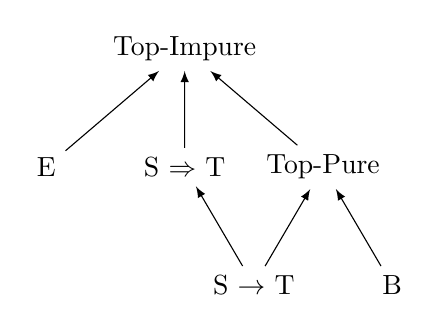
\begin{tikzpicture}[sibling distance=5em,
  every node/.style = {align=center},
  edge from parent/.style={draw,latex-}]
  \node {Top-Impure}
  child { node {E} }
  child { node (free) {S $\Rightarrow$ T} }
  child { node {Top-Pure}
    child { node (stoic) {S $\to$ T} }
    child { node {B} } };
  \path [draw, -latex] (stoic) -- (free);
\end{tikzpicture}

\caption{Subtyping: Top-Pure and Top-Impure}
\label{fig:stlc-impure-subtyping-tree}
\end{figure}

The second possibility is to keep the elegance of the type system and
changes the evaluation rules. We know that all terms of the type Top
are equivalent, because we can do nothing with a term of type Top. It
implies we can substitute them arbitrarily without changing the
meaning of the term. This observation inspires us to introduce a
\emph{top} value and change the standard \textsc{E-AppAbs} rule to two
evaluation rules as follows:

\infrule[E-AppAbs1]
{ T \neq Top }
{ (\lambda x:T.t_1) v_2 \longrightarrow [x \mapsto v_2]t_1 }

\infrule[E-AppAbs2]
{ T = Top }
{ (\lambda x:T.t_1) v_2 \longrightarrow [x \mapsto top]t_1 }

The two rules have the effect that if a function takes a parameter of
type Top, then when called it will drop the parameter and replace it
with the \emph{top} value. We follow this approach in the formulation
and the full definition is presented in
Figure~\ref{fig:stlc-impure-definition}.

\begin{figure}
\begin{framed}

% multi-column separator
\setlength{\columnseprule}{0.4pt}
\begin{multicols}{2}

\textbf{Syntax}

\begin{tabu} to \linewidth {l l l X[r]}
  t   & ::= &                    & terms:               \\
      &     & \colorbox{shade}{top} & top value            \\
      &     & x                  & variable             \\
      &     & $\lambda$ x:T.t    & abstraction          \\
      &     & t t                & application          \\
\\
  v   & ::= &                    & values:              \\
      &     & $\lambda$ x:T.t    & abstraction value    \\
      &     & x                  & variable value       \\
      &     & \colorbox{shade}{top}  & top value            \\
\\
  T   & ::= &                    & types:               \\
      &     & \colorbox{shade}{Top}  & top type             \\
      &     & B                  & basic type           \\
      &     & E                  & capability type      \\
      &     & T $\to$ T          & type of stoic funs       \\
      &     & \colorbox{shade}{T $\Rightarrow$ T} & type of free funs   \\
\end{tabu}

% \hfill\\
\vspace{0.1em}

\textbf{Evaluation} \hfill \framebox[1.2\width][r]{$t \longrightarrow t'$}

\infrule[E-App1]
{ t_1 \longrightarrow t'_1 }
{ t_1 \; t_2 \longrightarrow t'_1 \; t_2 }

\infrule[E-App2]
{ t_2 \longrightarrow t'_2 }
{ v_1 \; t_2 \longrightarrow v_1 \; t'_2 }

\infrule[E-AppAbs1]
{ \colorbox{shade}{$T \neq Top$} }
{ \colorbox{shade}{$(\lambda x:T.t_1) \; v_2 \longrightarrow [x \mapsto v_2]t_1$} }

\infrule[E-AppAbs2]
{ \colorbox{shade}{$T = Top$} }
{ \colorbox{shade}{$(\lambda x:T.t_1) \; v_2 \longrightarrow [x \mapsto top]t_1$} }

\textbf{Pure Environment}

\hfill

\begin{center}
\begin{tabular}{l c l}
pure($\varnothing$)                   & = &   $\varnothing$ \\
pure($\Gamma$, x: E)                  & = &  pure($\Gamma$) \\
\rowcolor{gray!40}
pure($\Gamma$, x: S $\Rightarrow$ T)  & = &  pure($\Gamma$) \\
pure($\Gamma$, x: T)                  & = &  pure($\Gamma$), x: T     \\
\end{tabular}
\end{center}

\columnbreak

\textbf{Typing}  \hfill \framebox[1.2\width][r]{$\Gamma \vdash x : T$}

\infax[T-Top]{ \colorbox{shade}{$\Gamma \vdash top : Top$} }

\infrule[T-Var]
{ x: T \in \Gamma }
{ \Gamma \vdash x : T }

\infrule[T-Abs1]
{ pure(\Gamma),\; x: S \vdash t_2 : T }
{ \Gamma \vdash \lambda x:S.t_2 : S \to T }

\infrule[T-Abs2]
{  \colorbox{shade}{$\Gamma,\; x: S \vdash t_2 : T$} }
{  \colorbox{shade}{$\Gamma \vdash \lambda x:S.t_2 : S \Rightarrow T$} }

\infrule[T-App]
{ \Gamma \vdash t_1 : S \to T \andalso \Gamma \vdash t_2 : S }
{ \Gamma \vdash t_1 \; t_2 : T }

\infrule[T-Sub]
{  \colorbox{shade}{$\Gamma \vdash t : S \andalso S <: T$} }
{  \colorbox{shade}{$\Gamma \vdash t : T$} }

\colorbox{shade}{\textbf{Subtyping}}  \hfill \framebox[1.2\width][r]{$S <: T$}

\infax[S-Top]{ T <: Top }

\infax[S-Refl]{ T <: T }

\infrule[S-Trans]
{ S <: U \andalso U <: T }
{ S <: T }

\infrule[S-Degen]
{ S \to T }
{ S \Rightarrow T }

\infrule[S-Fun1]
{ S1 <: S2 \andalso T2 <: T1 }
{ S2 \to T2 <: S1 \to T1 }

\infrule[S-Fun2]
{ S1 <: S2 \andalso T2 <: T1 }
{ S2 \Rightarrow T2 <: S1 \Rightarrow T1 }

\hfill\\

\end{multicols}
\end{framed}

\caption{System STLC-Impure}
\label{fig:stlc-impure-definition}
\end{figure}

Note that in this formulation, we need to change the definition of the
function \emph{pure} to exclude free function types in the pure
environment. This restriction is important, because we're not sure
what side effects there might be inside free functions. If we allow
stoic functions to have access to free functions, we'll loose the
ability to track the effects of stoic functions in the type system.

In principle, we can keep some free functions that we are sure can
never be called in the pure environment, such as
$(B \to E) \Rightarrow B$, as it's impossible to get an actual
instance of the type $B \to E$ in order to call this
function. However, from the perspective of practicity, it doesn't make
sense to have functions in the environment if they can never be
called. Thus, to simplify the system without sacrificing usability, we
removed all free function types from the pure environment.

\subsection{Soundness}

We proved both progress and preservation in Coq based on the
locally-nameless representation.

\begin{theorem}[Progress]
If $\varnothing \vdash t : T$, then either $t$ is a value or there is some
$t'$ with $t \longrightarrow t'$.
\end{theorem}

\begin{theorem}[Preservation]
If $\Gamma \vdash t : T$, and $t \longrightarrow t'$, then $\Gamma
\vdash t' : T$.
\end{theorem}

As you can imagine, now we need two different substitution lemmas in
the proof of perservation, corresponding to the two reduction rules.

\begin{lemma}[Subsitution-Not-Top]
  If $\Gamma,\; x:S \vdash t : T$, $S \neq Top$, s is a value and
  $\Gamma \vdash s : S$, then $\Gamma \vdash [x \mapsto s]t : T$.
\end{lemma}

\begin{lemma}[Subsitution-Top]
  If $\Gamma,\; x:Top \vdash t : T$, then $\Gamma \vdash [x \mapsto top]t : T$.
\end{lemma}

The reason why we restrict $s$ to be a value in the lemma
\emph{Substitution-Not-Top} is the same as we've seen in the system
STLC-Pure, thus we don't reiterate here.

\subsection{Effect Safety}

We follow the same approach as the system STLC-Pure in formulation of
effect safety. The formulation is an extension of the definition of
\emph{capsafe} and \emph{caprod} in STLC-Pure with free function
types.

\subsubsection{Formulation}

With the presence of free functions, the previous formulation of
effect safety is not enough. We not only need to ensure that it's
impossible to construct a term of the capability type in healthy
environments, but also need to ensure only stoic functions can be
called in healthy environments. The two conditions together guarantee
that there cannot be actual side effects inside a pure stoic
function. Thus, we need two statements about effect safety.

\begin{definition}[Effect-Safety-1]
  If $\Gamma$ is healthy, there doesn't exist $t$ with
  $\Gamma \vdash t : E$.
\end{definition}

\begin{definition}[Effect-Safety-2]
  If $\Gamma$ is healthy and $\Gamma \vdash t_1 \; t_2 : T$, then
  there exists U, V such that $\Gamma \vdash t_1 : U \to V$.
\end{definition}

A tempting formulation of the second effect safety statement would be
that in a healthy environment it's impossible to construct a term of
free function type. However, this formulation has no hope to be
proved, as $S \to T$ is a subtype of $S \Rightarrow T$, any term that
can be typed as the former can also be typed as the latter.

Now let's consider how to define \emph{capsafe} and \emph{caprod} for
free function types. Our first attempt is to add following rule:

\infax[CP-Fun2]{ S \Rightarrow T \quad caprod }

With this rule, the type $(B \Rightarrow B) \to E$ would be considered
\emph{capsafe}, according to the \textsc{CS-Fun1} rule. However, with
a variable $f$ of this type in the healthy environment, together with
another variable $g$ of the capsafe type $B \to B$, it's possible to
create the term \emph{f g}, which is of the capability type -- the
first statement of effect safety breaks. On ther other hand, we can't
do the opposite to take $S \Rightarrow T$ as \emph{capsafe}, as it
would allow calling free functions in healthy environments -- the
second statement of effect safety breaks.

This dilemma prompts us to reexamin the meaning of \emph{capsafe} and
\emph{caprod}. When these facilities were introduced in STLC-Pure,
they are formulated in terms of the provability of the capability type
E. From the perspective of provability of E, $S \to T$ and
$S \Rightarrow T$ don't make much difference. Thus, free functions
types should be formulated the same way as sotic function types. We
tried this approach, and it worked. The full formulation is presented
in Figure~\ref{fig:stlc-impure-healthy-definition}.

\begin{figure}[h]
\begin{framed}

% multi-column separator
\setlength{\columnseprule}{0.4pt}
\begin{multicols}{2}

\textbf{Capsafe}

\infax[CS-Base]
{ B \quad \text{capsafe} }

\infrule[CS-Fun1]
{ S \quad caprod }
{ S \to T \quad \text{capsafe} }

\infrule[CS-Fun2]
{ T \quad \text{capsafe} }
{ S \to T \quad \text{capsafe} }

\infrule[CS-Fun3]
{ \colorbox{shade}{$S \quad caprod$} }
{ \colorbox{shade}{$S \Rightarrow T \quad \text{capsafe}$} }

\infrule[CS-Fun4]
{ \colorbox{shade}{$T \quad \text{capsafe}$} }
{ \colorbox{shade}{$S \Rightarrow T \quad \text{capsafe}$} }

\columnbreak

\textbf{Caprod}

\infax[CP-Eff]
{ E \quad caprod }

\infrule[CP-Fun1]
{ S \; \text{capsafe} \andalso T \; caprod }
{ S \to T \quad caprod }

\infrule[CP-Fun2]
{ \colorbox{shade}{$S \; \text{capsafe} \andalso T \; caprod$} }
{ \colorbox{shade}{$S \Rightarrow T \quad caprod$} }

\textbf{Healthy}

\infax[H-Empty]
{ \varnothing \quad caprod }

\infrule[H-Var]
{ G \; healthy \andalso T \; \text{capsafe} }
{ G, \; x:T \quad healthy }

\hfill\\

\end{multicols}
\end{framed}

\caption{System STLC-Impure Healthy Environment}
\label{fig:stlc-impure-healthy-definition}
\end{figure}

\emph{Why this formulation of healthy environment is acceptable?} We
need to ensure that all inhabitable types that can
appear in the pure environment can also appear in the healthy
environment. This claim has been formally proved:

\begin{theorem}[Inhabitable-Capsafe]
  If the type T is inhabitable, then either T is capsafe or $T = E$ or
  T is a free function type.
\end{theorem}

From the theorem above, it's obvious that a pure environment $\Gamma$
with only variables of inhabitable types is also a healthy and pure
environment. Thus, any property proved for a healthy and pure
environment also holds for $\Gamma$.

A consequence of this definition that a healthy environment is no
longer pure. Conceptually speaking, a healthy environment should
always be a subset of the pure environment. However, this is not a
problem. We can define
$healthy' \; E := healthy \; E \wedge pure \; E = E$. Effect safety
proved only assuming \emph{healthy} also holds for $healthy'$. But
what's the purpose of defining such a weaker concept of
\emph{healthy}? The answer is that it makes the first statement of
effect safety simpler. As we'll see, the proof of the first statement
of effect safety only depends on \emph{healthy}, while the second
depends on \emph{healthy'}. Thus, we need a stronger version of the
second statement of effect safety:

\begin{definition}[Effect-Safety-2']
  If $\Gamma$ is healthy and pure, and $\Gamma \vdash t_1 \; t_2 : T$,
  then there exists U, V such that $\Gamma \vdash t_1 : U \to V$.
\end{definition}


\subsubsection{Proof}

The proof of the first statement of effect safety is almost the same
as in STLC-Pure. In the presence of subtyping, we need to add a
\emph{Capsafe-Sub} lemma.  The first effect safety statement follows
immediately from the lemma \emph{Healthy-Capsafe}.

\begin{lemma}[Capsafe-Not-Caprod]
 If type T is capsafe, then T is not caprod.
\end{lemma}

\begin{lemma}[Capsafe-Or-Caprod]
 For any T, T is either capsafe or caprod.
\end{lemma}

\begin{lemma}[Capsafe-Sub]
 If S is capsafe and $S <: T$, then T is capsafe.
\end{lemma}

\begin{lemma}[Healthy-Capsafe]
  If $\Gamma$ is healthy and $\Gamma \vdash t : T$, then T is capsafe.
\end{lemma}

\begin{theorem}[Effect-Safety-1]
  If $\Gamma$ is healhty, then there doesn't exist term $t$ with
  $\Gamma \vdash t : E$.
\end{theorem}

However, it's impossible to prove the second statement of effect
safety, which states that if we can construct an application
$t_1 \; t_2$ in a healthy and pure environment, then $t_1$ can be
typed as $S \to T$ for some S and T. To see an example why it cannot
be proved, let's assume
$\Gamma = \{f: B \to B \Rightarrow B, \; x: B\}$. It's obvious
$\Gamma$ is healthy and pure, however, $f \; x$ in the term
$(f \; x) \;x$ has the type $B \Rightarrow B$. And it's impossible to
prove that $f \; x$ has the type $B \to B$. If $f$ is not a variable,
but a fully defined function, then we can prove that $f$ also has the
type $B \to B \to B$. This is because the inner function of type
$B \Rightarrow B$ cannot capture any capabilities or free functions,
otherwise the outer function can't be typed as stoic!

This observation leads us to assume four well-founded axioms listed in
Figure~\ref{fig:stlc-impure-axioms}. These axioms can only be proved
if $\Gamma$ is empty\footnote{Except the axiom \textsc{Ax-Poly}, which
  cannot be proved even if $\Gamma$ is empty.}. Otherwise, if $t$ is a
variable, we can do nothing.

\begin{figure}[h]
\begin{framed}

% multi-column separator
% \setlength{\columnseprule}{0.4pt}
\begin{multicols}{2}

\infrule[Ax-Base]
{ \Gamma \vdash t : B \to S \Rightarrow T }
{ \Gamma \vdash t : B \to S \to T }

\hfill\\

\infrule[Ax-Top]
{ \Gamma \vdash t : Top \to S \Rightarrow T }
{ \Gamma \vdash t : Top \to S \to T }

\hfill\\

\infrule[Ax-Stoic]
{ \Gamma \vdash t : (U \to V) \to S \Rightarrow T }
{ \Gamma \vdash t : (U \to V) \to S \to T }

\hfill\\

\infrule[Ax-Poly]
{ \Gamma \vdash t_2 : U \to V \\
  \Gamma \vdash t_1 : (U \Rightarrow V) \to S \Rightarrow T }
{ \Gamma \vdash t_1 \; t_2 : S \to T }

\end{multicols}
\end{framed}

\caption{System STLC-Impure Axioms}
\label{fig:stlc-impure-axioms}
\end{figure}

The justification for the axiom \textsc{Ax-Base} is as
follows. Suppose $t = \lambda x:B. \; \lambda y:S. \; t_1$ and
$\Gamma \vdash t : B \to S \Rightarrow T$. The typing rule for $t$
should be the typing rule for stoic functions:

\infrule[Step-1]
{ pure(\Gamma),\; x: B \vdash \lambda y:S. \; t_1 : S \Rightarrow T }
{ \Gamma \vdash \lambda x:B. \lambda y:S. \; t_1 : B \to S \Rightarrow T }

Then what's the rule used in the typing of $\lambda y:S. \; t_1$? If
it's first typed as $S \to T$ and then subsumed as $S \Rightarrow T$,
then we are done. Otherwise, $\lambda y:S. \; t_1$ is typed using the
rule of free functions:

\infrule[Step-2]
{ pure(\Gamma),\; x: B,\; y:S \vdash t_1 : T }
{ pure(\Gamma),\; x: B \vdash \lambda y:S. \; t_1 : S \Rightarrow T }

According to the definition of \emph{pure}, we know that following two
equations holds:

\begin{itemize}
\item $pure(pure(\Gamma)) = pure(\Gamma)$
\item $pure(\Gamma, x:B) = pure(\Gamma), x:B$
\end{itemize}

From the equations above, we can get following equation:

\begin{center}
  $pure(pure(\Gamma),\; x: B) = pure(\Gamma),\; x: B$
\end{center}

If we substitute the equation in Step-2, we get exactly the
precondition for typing stoic functions. Thus $\lambda y:S.t_2$ can be
typed as stoic function:

\infrule[Step-2']
{ pure(pure(\Gamma),\; x: B),\; y:S \vdash t_1 : T }
{ pure(\Gamma),\; x: B \vdash \lambda y:S. \; t_1 : S \to T }

Because we know $\lambda y:S. \; t_1$ is typed as $S \to T$, so we can
update Step-1 as following:

\infrule[Step-1']
{ pure(\Gamma),\; x: B \vdash \lambda y:S. \; t_1 : S \to T }
{ \Gamma \vdash \lambda x:B. \lambda y:S. \; t_1 : B \to S \to T }

Put all the steps together, we obtained
$\Gamma \vdash t : B \to S \to T$ from the fact
$\Gamma \vdash t : B \to S \Rightarrow T$. That's the justification
for the \textsc{Ax-Base} rule. The justifications for \textsc{Ax-Top}
and \textsc{Ax-Stoic} are similar. The axiom \textsc{Ax-Poly} is an
interesting one, which deserves a separate section.

Assuming the axioms above, it's straight-forward to prove a lemma
\emph{Healthy-Pure-Stoic}, and the second statement of effect safety
follows immediately from the lemma.

\begin{lemma}[Healthy-Pure-Stoic]
  If $\Gamma$ is healthy and pure,  and $\Gamma \vdash t : S
  \Rightarrow T$, then $\Gamma \vdash t : S \to T$.
\end{lemma}

\begin{theorem}[Effect-Safety-2']
  If $\Gamma$ is healthy and pure, and $\Gamma \vdash t_1 \; t_2 :
  T$, then there exists U, V such that $\Gamma \vdash t_1 : U \to V$.
\end{theorem}

Note that unlike the proof of the first effect safety statement, the
proof of the second statement of effect safety assumes that $\Gamma$
is pure. This is due to the fact that \emph{healthy} no longer implies
\emph{pure}. Conceptually speaking, a healthy environment should
always be a subset of pure environment. To clear the worry of readers,
we can define $healthy' \; E := healthy \; E \wedge pure \; E = E$.
The first statement of effect safety is proved only assuming the
weaker \emph{healthy}, it certainly holds for $healthy'$ as well.

\subsection{Effect Polymorphism}

The axiom \textsc{Ax-Poly}, which we call \emph{effect polymorphism},
reflects some important property about capability-based effect
systems.

\infrule[Ax-Poly] { \Gamma \vdash t_2 : U \to V \andalso \Gamma \vdash
  t_1 : (U \Rightarrow V) \to S \Rightarrow T } { \Gamma \vdash t_1 \;
  t_2 : S \to T }


Suppose following typing relation holds, what impure
variables can be captured by $t_1$?

\begin{center}
  $\Gamma \vdash \lambda f:U \Rightarrow V. \; \lambda y:S. \; t_1 : (U
  \Rightarrow V) \to S \Rightarrow T$.
\end{center}

As the functioin is stoic, the only impure variable can be captured is
$f$. Now, if we supply a stoic function as parameter to the function,
it has the same effect as saying that $f$ is $U \to V$. Thus in this
context, the function can be typed as $(U \to V) \to S \Rightarrow T$.
Now according to the \textsc{Ax-Stoic} axiom, the term can also be
typed as $(U \to V) \to S \to T$. Then according to the standard
\textsc{T-App} rule, the type of the application is $S \to T$. That's
the justification for the axiom \textsc{Ax-Poly}.

Effect polymorphism is an advantage of capability-based effect systems
over monad-based effect systems. In Haskell, there is always the need
to maintain two copies of higher-order functions, as following code
snippet shows\footnote{From the slides of Ben Lippmeier,
  \emph{Witnessing Purity, Constancy and Mutability}, APLAS 2009}:

\begin{lstlisting}[language=Haskell]
  map :: (a -> b) -> List a -> List b
  map f xs
    = case xs of
        Nil -> Nil
        Cons x xs -> Cons (f x) (map f xs)

  mapIO :: (a -> IO b) -> List a -> IO (List b)
  mapIO f xs
    = case xs of
      Nil -> return Nil
      Cons x xs -> do x' <- f x
        xs' <- mapIO f xs
        return (Cons x' xs')
\end{lstlisting}

The non-monadic version and the monadic version of code are the same
in essence. It's a pity that we have to duplicate the same code twice
in monad-based effect systems. In capability-based effect systems, we
only need to maintain one copy of the code:

\begin{lstlisting}[language=Scala]
  def map[A,B](f: A => B)(l: List[A]) = l match {
    case Nil => Nil
    case x::xs => f(x)::map(f)(l)
  }
\end{lstlisting}
% haskell two versions of map

The \emph{map} function above has the type
$(A \Rightarrow B) \to List[A] \Rightarrow List[B]$. Is \emph{map} a
pure function? It depends on how it's used. When supplied with a
function of type $A \Rightarrow B$ with side effects, \emph{map} is
impure. When supplied with a pure function $f$ of type $A \to B$,
\emph{map} has the actual type $(A \to B) \to List [A] \to List[B]$,
thus is pure. Following code snippet demonstrates the usage of
\emph{map} in both pure and impure settings.

\begin{lstlisting}[language=Scala]
  def squareImpure(list: List[Int])(c: IO) = {
    map { x => println(x)(c); x*x } list
  }

  def squarePure(list: List[Int]) = {
    map { x => x*x } list
  }
\end{lstlisting}

In the code above, the lambda passed to \emph{map} in
\emph{squareImpure} is not stoic, as it captures the capability
$c$. The function \emph{squareImpure} has the type
$List[Int] \to IO \to List[Int]$, and \emph{squarePure} has the type
$List[Int] \to List[Int]$. This means all effects are captured in the
type system even in the presence of (local) free functions.

The reader might be wondering, what if we want to stipulate that the
passed function \emph{f} can only have IO effects? How does effect
polymorphism work in such cases? The answer is as follows:

\begin{lstlisting}[language=Scala]
  private def mapImpl[A,B](f: A => B)(l: List[A]) = l match {
    case Nil => Nil
    case x::xs => f(x)::map(f)(l)
  }

  def map[A,B](f: A -> B) = mapImpl(f)

  def map[A,B](c: IO)(f: IO -> A => B) = mapImpl(f c)
\end{lstlisting}

In the above, we only have one implementation of the \emph{map}
function and we protect the implementation with the keyword
\emph{private}. All callings of the \emph{map} function has to go
through the two exposed interface. The two interfaces imposes that the
passed function \emph{f} must either be pure or only have IO side
effects. And it's possible to add new interfaces to allow more effects
without breaking compatibility of existing code. This is the power and
flexibility of capability-based effect systems.

\section{Conclusion}

We've seen that the existence of \emph{stoic functions} is the main
trait of capability-based effect systems. The interplay between
\emph{stoic functions} and \emph{free functions} enables flexible
programming patterns that trivially solve the problem of \emph{effect
  polymorphism}.

Capability-based effect systems have to be paired with strict
evaluation, just like monad-based effect systems have to be paired
with lazy evaluation.

In the two proposed systems with universal types, namely F-Pure and
F-Impure, it's impossible to abstract over capability types.

\subsection{Related Work}

Lucassen and Gifford first introduced type-and-effect
systems\cite{gifford1986integrating} and effect polymorphism using
effect type parameterization \cite{lucassen1988polymorphic}, which is
further developed by Talpin and Jouvelot to provide type-and-effect
inference \cite{talpin1992polymorphic, talpin1994type}.

Moggi introduced the usage of monads for computation
effects\cite{moggi1991notions}. Wadler popularized the usage of
monads\cite{wadler1992comprehending, wadler1995monads} and proved that
it's possible to transpose any type-and-effect system into a
corresponding monad system\cite{wadler2003marriage}. Lippmeier
proposed the usage of region variables and dependently kinded witness
to encode mutability polymorphism\cite{lippmeier2009witnessing}.

Lukas \emph{et al.}  studied type-and-effect system for
Scala\cite{rytz2012lightweight, rytz2013flow, lukas2014effect}.  In
lightweight polymorphic effects\cite{rytz2012lightweight}, the
dichotomy between \emph{effect-polymorphic function type} and
\emph{monomorphic function type} resembles the dichotomy between
\emph{stoic function types} and \emph{free function types}.  They
unified the two function types in a framework called \emph{relative
  effect annotation} based on dependent types. They also implemented a
plugin for the Scala compiler.

Heather \emph{et al.} proposed a special function type called
\emph{spores} for Scala\cite{miller2014spores}. Compared to normal
functions, spores observe a variable capturing discipline. The set of
types allowed or not allowed to be captured is part of the type
signature of spores, and can be flexibly customized by
programmers. Spores are well suited for distributed and parallel
computations, but don't generalize to a practical effect system.

Crary \emph{et al.} proposed a capability calculus for typed
region-based memory management\cite{crary1999typed}. The safety of
deallocation of memory can be guaranteed by the type system. In the
capability calculus, capabilities are sets of regions that are
presently valid to access, in contrast to the abstract meaning of
capabilities in our systems. The difference is mainly due to the
different focus of effects under study.

\subsection{Future Work}

One approach to make parametric polymorphism work for capability types
is to integrate \emph{bounded quantification} with capabilities. This
is the what we are working on now. We've managed to prove soundness of
the system, and the proof of effect safety is in progress.

Another direction of work is to extend the proposed systems with some
implicit calculus, in order to avoid explicitly passing capabilities
around in the code. This would result in significant savings in
boilerplate code, thus make the system more friendly to programmers.

The most exciting work would be to implement a capability-based type
system in Scala or other industrial programming languages and
popularize the usage of effect systems in the programming community.


%now enable appendix numbering format and include any appendices
%% \appendix
%% \include{content/appendix1}

%next line adds the Bibliography to the contents page
\addcontentsline{toc}{section}{Bibliography}
%uncomment next line to change bibliography name to references
%\renewcommand{\bibname}{References}
\bibliography{refs}        %use a bibtex bibliography file refs.bib
\bibliographystyle{plain}  %use the plain bibliography style

\end{document}
